\documentclass[aspectratio=169,11pt]{beamer}

\usetheme{Cuhksz}

\usepackage{amsmath,amssymb}
\usepackage{booktabs}
\usepackage{graphicx}

\graphicspath{{../figures/}}

\cuhkszlogopath{assets/cuhksz_logo_alt.png}
\cuhkszwordmarkpath{assets/cuhksz_wordmark.png}
\cuhkszsetfooterleft{CUHK-Shenzhen}
\cuhkszsetfootercenter{XUE Yantong}

% Arrange author names and placeholder emails in equally sized columns.
\newcommand{\cuhkszcoverrow}[3]{%
  \begin{tabular}{@{}c@{\hspace{0.20cm}}c@{\hspace{0.20cm}}c@{}}
    \makebox[4.35cm][l]{#1} & \makebox[4.35cm][l]{#2} & \makebox[4.35cm][l]{#3}
  \end{tabular}}

\title[Weather and bike-share usage]{Weather sensitivity of bike-share usage\\a hierarchical Bayesian plan for 25 cities}
\subtitle{STA5001 Bayesian \& Computational Statistics}
\author{\small\cuhkszcoverrow
  {XUE Yantong}{WANG Ziyu}{ZHAO Jiashen}}
\institute{\footnotesize\cuhkszcoverrow
  {student1@example.com}{student2@example.com}{student3@example.com}}
\date{STA5001 \textperiodcentered\ 3 November 2026}
\hypersetup{
  pdftitle={Weather sensitivity of bike-share usage: a hierarchical Bayesian plan for 25 cities},
  pdfauthor={XUE Yantong, WANG Ziyu, and ZHAO Jiashen},
}

\newcommand{\hl}[1]{{\color{csPurple}\bfseries #1}}
\newcommand{\hlg}[1]{{\color{csGold}\bfseries #1}}

\begin{document}

% ---------------------------------------------------------------- Cover
\begin{frame}[plain,noframenumbering]
  \titlepage
\end{frame}

% ---------------------------------------------------------------- 1
\begin{frame}{Weather drives bike-share usage}
  \small
  \begin{columns}[T,onlytextwidth]
    \begin{column}{0.50\textwidth}
      \textbf{The reference study.} Bean, Pojani and Corcoran (2021) compare
      \hl{forty cities} across climate zones, fitting a separate generalized
      additive model to each.

      \vspace{0.30cm}
      Two robust patterns: hires rise with UTCI up to about
      \hlg{27--28\,$^\circ$C} and then fall; rainfall is associated with lower use.
    \end{column}
    \begin{column}{0.46\textwidth}
      \begin{alertblock}{What a per-city fit cannot answer}
        \begin{itemize}
          \item How much cities differ --- no quantity describes the spread.
          \item Small systems are estimated noisily.
        \end{itemize}
      \end{alertblock}
      \vspace{0.20cm}
      \textbf{Question.} Do a city's thermal and rainfall background explain
      part of its weather sensitivity?
    \end{column}
  \end{columns}
\end{frame}

% ---------------------------------------------------------------- 2
\begin{frame}{Data: one public release, 29 reproducible cities}
  \small
  \begin{columns}[T,onlytextwidth]
    \begin{column}{0.52\textwidth}
      \begin{block}{Source}
        \begin{tabular}{@{}p{2.2cm}p{4.2cm}@{}}
          Release & Mendeley Data, CC BY 4.0 \\[0.2em]
          DOI & \texttt{10.17632/2nxpvtz935.1} \\[0.2em]
          Content & hourly hires, UTCI, rainfall \\[0.2em]
          Scope & 29 dock-based systems
        \end{tabular}
      \end{block}
    \end{column}
    \begin{column}{0.44\textwidth}
      \textbf{Why 29 and not 40.} The paper's own code designates the dock-based
      systems; the other cities have metadata but no hourly stock data.

      \vspace{0.28cm}
      Each city contributes exactly \hl{8{,}760} hourly rows.
    \end{column}
  \end{columns}
  \vspace{0.30cm}
  \centering
  \footnotesize Archive and paper are both stored with SHA-256 digests, re-checked on every run.
\end{frame}

% ---------------------------------------------------------------- 3
\begin{frame}{From hourly records to 9{,}120 analysis days}
  \small
  \begin{columns}[T,onlytextwidth]
    \begin{column}{0.47\textwidth}
      \begin{block}{Processing}
        \begin{itemize}
          \item Preserve row order, map onto consecutive UTC hours
          \item Convert to the city's local time zone
          \item Aggregate by local date
        \end{itemize}
      \end{block}
    \end{column}
    \begin{column}{0.49\textwidth}
      \begin{block}{Quality rules}
        \begin{itemize}
          \item 23--25 hourly rows per local day
          \item at least 20 valid UTCI hours
          \item complete precipitation
        \end{itemize}
      \end{block}
    \end{column}
  \end{columns}
  \vspace{0.34cm}
  \centering
  \footnotesize
  254{,}040 hourly rows $\rightarrow$ 10{,}613 candidate city-days $\rightarrow$
  \hl{10{,}578} kept $\rightarrow$ \hl{9{,}120} in the primary sample of 25 cities
  \par\vspace{0.18cm}
  \footnotesize Three repeated time keys exist; Dublin and Melbourne coincide with daylight-saving
  transitions, Brisbane does not observe daylight saving; the paper's row-order rule is kept.
\end{frame}

% ---------------------------------------------------------------- 4
\begin{frame}{Cities differ in scale by four orders of magnitude}
  \begin{center}
    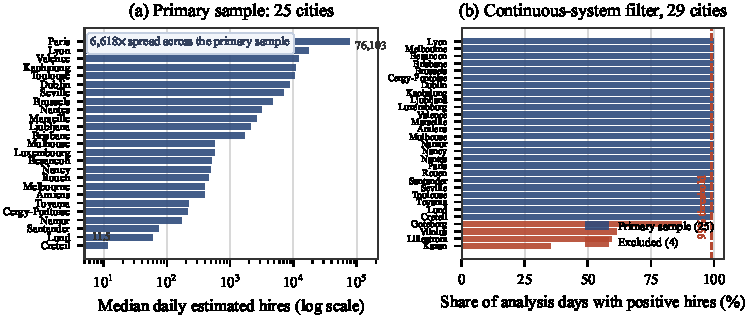
\includegraphics[width=0.94\textwidth,height=4.6cm,keepaspectratio]{report_fig1_data_overview.pdf}
  \end{center}
  \vspace{-0.25cm}
  \centering
  \small Median daily hires run from \hlg{11.5} in Cr\'eteil to \hlg{76{,}103} in Paris.
  \par\vspace{0.12cm}
  \footnotesize The four cities below the 99\% line are excluded from the primary sample.
\end{frame}

% ---------------------------------------------------------------- 5
\begin{frame}{Thermal response peaks near 27.5\,$^\circ$C}
  \begin{center}
    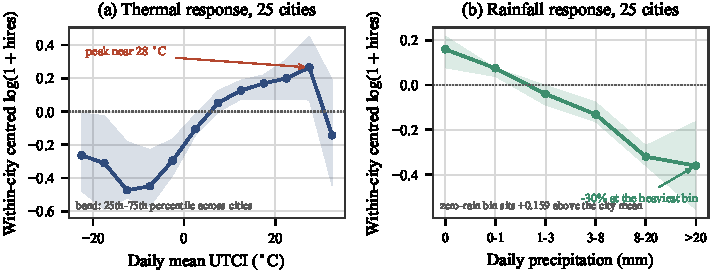
\includegraphics[width=0.94\textwidth,height=4.6cm,keepaspectratio]{report_fig2_weather_usage.pdf}
  \end{center}
  \vspace{-0.25cm}
  \centering
  \small Peaks at \hlg{+0.26} near \hl{27.5\,$^\circ$C}, then falls to $-0.14$ in the hottest bin.
  \par\vspace{0.12cm}
  \footnotesize Rainfall declines monotonically: the heaviest bin sits about \hlg{41\%} below the dry bin.
\end{frame}

% ---------------------------------------------------------------- 6
\begin{frame}{Season and week disagree across cities}
  \begin{center}
    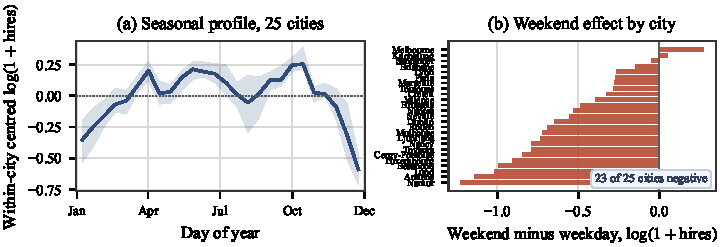
\includegraphics[width=0.94\textwidth,height=4.4cm,keepaspectratio]{report_fig3_seasonality.pdf}
  \end{center}
  \vspace{-0.25cm}
  \centering
  \small The seasonal amplitude of \hlg{0.84} log units exceeds the whole thermal effect.
  \par\vspace{0.12cm}
  \footnotesize 23 of 25 cities have lower weekend use; Melbourne is the only clearly positive city.
\end{frame}

% ---------------------------------------------------------------- 7
\begin{frame}{Plan: one hierarchy instead of 25 separate fits}
  \small
  \begin{columns}[T,onlytextwidth]
    \begin{column}{0.54\textwidth}
      \textbf{Response.} $y_{it}=\log(1+U_{it})$, Student-$t$ observation
      distribution with estimated degrees of freedom.

      \vspace{0.24cm}
      \textbf{Location.} city intercept, thermal anomaly and its square,
      standardised rainfall, weekend, annual sine and cosine.

      \vspace{0.24cm}
      \textbf{Hierarchy.} city coefficients share a normal population
      distribution, written in non-centred form.
    \end{column}
    \begin{column}{0.42\textwidth}
      \begin{block}{What this buys}
        \begin{itemize}
          \item Between-city spread is an estimated quantity
          \item Population means vary with city climate background
          \item Low-volume systems borrow strength
        \end{itemize}
      \end{block}
      \vspace{0.18cm}
      \footnotesize NUTS via PyMC and nutpie, four chains of 2{,}000 draws.
    \end{column}
  \end{columns}
\end{frame}

% ---------------------------------------------------------------- 8
\begin{frame}{Take-away}
  \vspace{0.24cm}
  \begin{enumerate}
    \setlength{\itemsep}{0.52cm}
    \item A reproducible panel of \hl{25 cities and 9{,}120 city-days} is frozen
      and documented.
    \item The thermal response is \hl{non-monotone}, peaking near
      \hlg{27.5\,$^\circ$C}, and rainfall is associated with monotonically lower use.
    \item Cities differ in scale, in weekend behaviour and in their weather
      response --- which is why the final model is a \hl{hierarchy}.
  \end{enumerate}
  \vspace{0.60cm}
  \centering \hl{Questions}
\end{frame}

% ================================================================ backup
\begin{frame}{Backup: filtering and sample construction}
  \footnotesize
  \begin{tabular}{@{}p{5.0cm}p{7.4cm}@{}}
    \toprule
    \textbf{Stage} & \textbf{Result} \\
    \midrule
    Hourly stock rows for 29 cities & 254{,}040 \\
    Candidate local days & 10{,}613 \\
    Days failing a quality rule & 35 \\
    Retained city-days & 10{,}578 \\
    Cities recording hires on $\ge 99\%$ of days & 25 \\
    Primary sample & 9{,}120 city-days \\
    \bottomrule
  \end{tabular}
  \vspace{0.40cm}

  Exclusions overlap: 28 days outside the nominal study period, 34 outside the
  23--25 hour count, 33 short of 20 UTCI hours, none on precipitation.
  The four excluded cities are G\"oteborg, Kazan, Lillestr\o m and Vilnius.
\end{frame}

\begin{frame}{Backup: model and priors}
  \footnotesize
  \begin{columns}[T,onlytextwidth]
    \begin{column}{0.50\textwidth}
      \begin{block}{Priors on the $\log(1+U)$ scale}
        \begin{tabular}{@{}ll@{}}
          Population intercept & $\mathcal{N}(7,2)$ \\
          City intercept scale & HN$(2)$ \\
          Thermal, per 10\,$^\circ$C & $\mathcal{N}(0,0.5)$ \\
          Quadratic & $\mathcal{N}(0,0.3)$ \\
          Rainfall & $\mathcal{N}(0,0.3)$ \\
          Weekend & $\mathcal{N}(0,0.4)$ \\
          Seasonal & $\mathcal{N}(0,0.8)$ \\
        \end{tabular}
      \end{block}
    \end{column}
    \begin{column}{0.46\textwidth}
      Degrees of freedom $\nu=2+\text{Exponential}(0.1)$; moderator coefficients
      use $\mathcal{N}(0,0.2)$ to $\mathcal{N}(0,0.3)$, and city scales use
      HalfNormal priors matched to the population scale.

      \vspace{0.30cm}
      A prior predictive check will verify the implied range of daily hires and
      weather multipliers before the observed outcomes are examined.

      \vspace{0.30cm}
      Convergence thresholds: $\widehat{R}\le 1.01$, bulk and tail ESS at 400,
      no divergences.
    \end{column}
  \end{columns}
\end{frame}

\begin{frame}{Backup: per-city curves for six representative cities}
  \footnotesize
  \begin{columns}[T,onlytextwidth]
    \begin{column}{0.49\textwidth}
      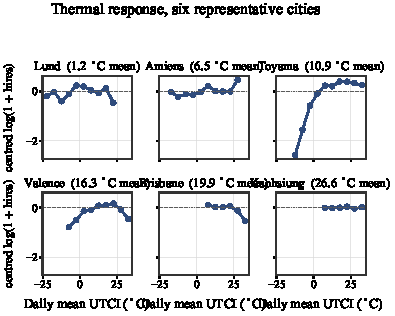
\includegraphics[width=\textwidth,height=4.4cm,keepaspectratio]{figS8_utci_curves_selected.pdf}
    \end{column}
    \begin{column}{0.49\textwidth}
      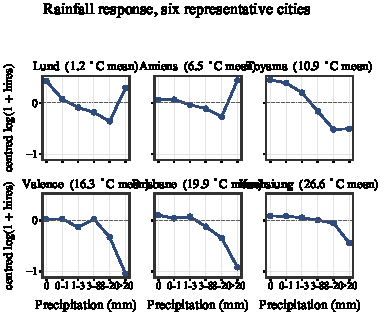
\includegraphics[width=\textwidth,height=4.4cm,keepaspectratio]{figS9_rain_curves_selected.pdf}
    \end{column}
  \end{columns}
  \vspace{0.16cm}
  \centering
  Lund (1.2\,$^\circ$C), Amiens (6.5), Toyama (10.9), Valence (16.3), Brisbane
  (19.9) and Kaohsiung (26.6) are equally spaced over the range of city means;
  the grids for all 25 cities are in the supplementary figures.
\end{frame}

\begin{frame}{Backup: source and reproducibility}
  \footnotesize
  \begin{itemize}
    \setlength{\itemsep}{0.14cm}
    \item Data release: Mendeley Data, DOI \texttt{10.17632/2nxpvtz935.1},
      CC BY 4.0, Version 1.
    \item Reference paper: Bean, Pojani and Corcoran (2021),
      \emph{Journal of Transport Geography} 95:103155.
    \item Preparation: \texttt{python code/prepare\_bikeshare\_weather.py}
    \item Daily panel: \texttt{data/clean/bikeshare\_weather\_daily.csv},
      10{,}578 rows $\times$ 28 columns.
    \item Pilot model: \texttt{code/run\_pilot\_model.sh}, PyMC 6.3.2 with
      nutpie. No divergences, but several city-level parameters mixed poorly and
      some transitions hit the maximum tree depth, so it is a feasibility test.
    \item Verification: \texttt{python code/verify\_project\_setup.py}
  \end{itemize}
\end{frame}

\end{document}
